\documentclass{article}

\usepackage{hyperref}                 % Hyperlinks
\hypersetup{
	hidelinks,                        % Hide link boxes
	colorlinks = true,
	citecolor = cyan,
	urlcolor = black,
	linkcolor = magenta
}
\usepackage{arxiv}
\usepackage{amsmath}
\usepackage[utf8]{inputenc} % allow utf-8 input
\usepackage[T1]{fontenc}    % use 8-bit T1 fonts
\usepackage{url}            % simple URL typesetting
\usepackage{booktabs}       % professional-quality tables
\usepackage{amsfonts}       % blackboard math symbols
\usepackage{nicefrac}       % compact symbols for 1/2, etc.
\usepackage{microtype}      % microtypography
\usepackage{cleveref}       % smart cross-referencing
\usepackage{lipsum}         % Can be removed after putting your text content
\usepackage{graphicx}
\usepackage{natbib}
\usepackage{doi}
\usepackage{xcolor}
\usepackage{enumerate}% http://ctan.org/pkg/enumerate
\usepackage{float}

\usepackage{subcaption}


\title{Amortized Inference for Multiscale Hybrid Models of Infectious Disease}

\renewcommand{\shorttitle}{Amortized Inference for Multiscale Models}

\newcommand{\todo}[1]{\textcolor{red}{\textbf{[TODO: #1]}}}


% Here you can change the date presented in the paper title
%\date{September 9, 1985}
% Or remove it
%\date{}


% Multiple affiliations variant of author block
\usepackage{authblk}
\renewcommand\Authfont{\bfseries}
\setlength{\affilsep}{0em}
% box is needed for correct spacing with authblk
\newbox{\orcid}\sbox{\orcid}{
\includegraphics[scale=0.06]{orcid.pdf}}

\author[1,2]{%
	\href{https://orcid.org/0000-0002-6542-6032}{\usebox{\orcid}\hspace{1mm}Tom Kimpson\thanks{Corresponding author: \texttt{tom.kimpson@unimelb.edu.au}}}%
}

\author[1]{%
	\href{https://orcid.org/0000-0002-0556-1080}{\usebox{\orcid}\hspace{1mm}Ifrah Saeed }%
}

\author[1]{%
	\href{https://orcid.org/0000-0000-0000-0000}{\usebox{\orcid}\hspace{1mm}Domenic Germano}%
}

\author[1,2]{%
	\href{https://orcid.org/0000-0002-8809-726X}{\usebox{\orcid}\hspace{1mm}Jennifer Flegg}%
}
\author[2,3]{%
	\href{https://orcid.org/0000-0000-0000-0000}{\usebox{\orcid}\hspace{1mm}Mark Flegg }%
}

\affil[1]{School of Mathematics and Statistics, The University of Melbourne, Parkville, VIC 3010, Australia}
\affil[2]{ARC Centre of Excellence for the Mathematical Analysis of Cellular Systems (MACSYS), The University of Melbourne, Parkville, VIC 3010, Australia }
\affil[3]{Monash...}




% Uncomment to override  the `A preprint' in the header
%\renewcommand{\headeright}{Technical Report}
\renewcommand{\undertitle}{}


%%% Add PDF metadata to help others organize their library
%%% Once the PDF is generated, you can check the metadata with
%%% $ pdfinfo template.pdf
%\hypersetup{
%pdftitle={Amortized Inference for Stochastic Biological Models using Neural Posterior Estimation},
%pdfsubject={q-bio.NC, q-bio.QM},
%pdfauthor={David S.~Hippocampus, Elias D.~Striatum},
%pdfkeywords={First keyword, Second keyword, More},
%}

\begin{document}
\maketitle





\begin{abstract}
Multiscale infectious disease models are essential for capturing the interplay between large-scale deterministic population growth and small-scale stochastic events, such as viral extinction. While hybrid simulation frameworks like Jump-Switch-Flow (JSF) efficiently handle these dynamics, calibrating them to noisy clinical data remains a significant computational bottleneck. Traditional likelihood-free inference methods, such as Sequential Monte Carlo (SMC), are computationally intensive "online" algorithms that scale linearly with cohort size, rendering them impractical for real-time clinical intervention or large-scale epidemiological surveillance. In this work, we overcome this barrier by coupling hybrid simulation with Neural Posterior Estimation (NPE). This approach amortizes the computational cost by training a neural network to approximate the posterior distribution offline, allowing for near-instantaneous inference on new data. Using the Target-cell, Eclipsed-cell, Infectious-cell, Refractory-cell, Virion (TEIRV) model of within-host viral dynamics as a case study, we demonstrate that the JSF-NPE framework reduces inference latency from hours to less than one second per patient. Furthermore, we show that NPE matches the accuracy of gold-standard particle filters while superiorly resolving multimodal posterior landscapes and late-stage dynamics, features that sequential methods frequently miss due to mode collapse and particle degeneracy. By resolving the trade-off between model complexity and inference speed, this framework enables the deployment of sophisticated stochastic models in time-critical medical decision-making and population-level analysis.
\textcolor{red}{TK: key point is that simulation (i.e. JSF) is only half of the challenge. We also need to calibrate these models to data. ALSO, there are some cases where we want to calibrate these models to data \textit{rapidly}}
\end{abstract}


% keywords can be removed
%\keywords{First keyword \and Second keyword \and More}

\section{Introduction}\label{sec:introduction}

Infectious disease models must capture biological processes that span vastly different scales. In within-host viral dynamics, populations may grow to billions of particles, yet clinically critical events like pathogen clearance occur when particle counts are low. Comparable multiscale challenges arise in between-host transmission: a single infected individual may seed an outbreak affecting thousands, or an infection chain may stochastically fade to extinction before establishing itself \cite{Anderson1991Infections, Perelson2002Modelling, Baccam2006Influenza}. Accurately modelling these systems requires representing both large-scale dynamics efficiently and small-scale stochastic events faithfully \cite{Isaacson2013, Flegg2014, Cotter2016}. Continuous, deterministic models, such as Ordinary Differential Equations (ODEs), are computationally efficient and work well when populations are large. However, they are inaccurate when populations are small,  lacking absorbing states to capture extinction events, and leading to ``atto-fox" type problems where populations become unphysically small \cite{Fowler2021Attofox, Mollison1991Attofox, Lobry2015Attofox}. Conversely, discrete stochastic models like Continuous Time Markov Chains (CTMCs) naturally capture extinction and other rare events, but become computationally intractable when populations are large.

Hybrid simulation methods such as the Jump-Switch-Flow (JSF) framework \cite{Germano2024JSF}, resolve this conflict by dynamically coupling deterministic ODEs for high-occupancy states with stochastic CTMCs for low-occupancy states. This approach retains computational efficiency at large scales while preserving the essential stochastic behaviors that dominate at small scales. Hybrid methods like JSF have been successfully applied to within-host viral models, demonstrating accurate and efficient simulation of multiscale dynamics.
However, forward simulation is only part of the challenge. To be clinically or epidemiologically useful, the inverse problem must be solved; calibrating models to observed data, typically by inferring parameters from noisy, incomplete time series. 

Traditionally, the posterior distributions for these hybrid models are estimated using Simulation-Based Inference (SBI) techniques \cite{Cranmer2020NPE}. The most common approaches include sequential Monte Carlo methods, such as particle filters 
\cite{Arulampalam2002PF, Kitagawa1996PF} or Approximate Bayesian Computation (ABC) \cite{ABC}.
The original JSF framework, for instance, demonstrated parameter inference using particle filters. While theoretically capable, these methods are computationally intensive ``online" algorithms that require thousands of model simulations to generate a single posterior. This cost is not amortised; it must be paid separately for every new dataset. Consequently, analysing a single patient's viral load trajectory might require hours of computation; analysing a cohort of hundreds of patients becomes prohibitively expensive. Additionally, the efficiency of these methods degrades rapidly in complex scenarios, often struggling with high-dimensional problems, particle degeneracy (in particle filters) or difficulties with tuning tolerance thresholds and selecting appropriate summary statistics (in ABC). 



This computational bottleneck limits the practical utility of hybrid models in two critical settings. First, in time-sensitive intervention scenarios, the primary constraint is latency. In these contexts, the speed of inference per case is paramount; slow methods render results obsolete for immediate intervention. For example, optimising an antiviral regimen for an immunocompromised ICU patient requires parameter inference within minutes of data collection, not hours. Second, in large-scale epidemiological analyses, the limiting factor is throughput. Here, the cumulative cost of performing slow, serial inference across a cohort becomes prohibitive. This hinders population-level tasks such as monitoring drug resistance in adaptive clinical trials or informing culling strategies during widespread animal epidemics, where insights depend on synthesizing dynamics from hundreds or thousands of infection chains.



In this paper, we address this computational challenge by replacing sequential inference methods with Neural Posterior Estimation (NPE), an SBI technique that amortizes the cost of parameter estimation \cite{Papamakarios2016NPE, Greenberg2019NPE, Cranmer2020NPE}. NPE trains a neural network, typically a normalizing flow conditioned on time-series data, to directly approximate the mapping from observed data to posterior parameter distributions. This approach inverts the traditional inference paradigm: instead of running many simulations for each new dataset, we run many simulations once during an offline training phase. After training, generating posterior estimates for new data becomes computationally trivial, often requiring only seconds on standard hardware.

We demonstrate this JSF-NPE framework using the Target-cell, Eclipsed-cell, Infectious-cell, Refractory-cell, Virion (TEIRV) model of within-host viral dynamics as a case study. This model exemplifies the multiscale challenges that motivate our approach: viral populations span many orders of magnitude, and stochastic extinction (viral clearance) is the primary clinical outcome of interest. We show that NPE achieves accuracy comparable to particle filter methods while reducing per-patient inference time by several orders of magnitude---from hours to seconds. This performance gain makes hybrid stochastic models practical for time-sensitive clinical applications and enables large-scale epidemiological analyses that were previously computationally infeasible.

This paper is organised as follows. In Section \ref{sec:sim_methods}, we review simulation methods for multiscale systems. Section \ref{sec:inference_methods} outlines inference methods for multiscale systems, including NPE. In Section \ref{sec:TEIRV}, we introduce the TEIRV model used as a case study. Finally, the results of the JSF-NPE pipeline are presented in Section \ref{sec:results}. 

%%%%%%%%%%%%%%%%%%%%%%%%%%%%%%%%%%%%%%%%%%%%%%%%%%%%%%%%%%%%%%%%%%%%%%%%%%%%%%%%
\section{Simulation Methods}\label{sec:sim_methods}


Simulating multiscale viral dynamics requires choosing between deterministic efficiency and stochastic fidelity. Deterministic models based on ODEs represent the standard approach for large-scale dynamics. These models describe the time-evolution of mean species populations via reaction rate equations. While numerical integration methods for ODEs are mature and highly efficient~\cite{griffiths2010numerical}, this mean-field approximation assumes large population sizes where fluctuations average out. Consequently, ODEs break down when populations are small: they allow for unphysical fractional individuals and lack absorbing states, rendering them incapable of naturally modelling extinction events or stochastic fade-out.

To capture these discrete, stochastic effects, the system can be modelled as a Continuous Time Markov Chain (CTMC). Simulating CTMCs requires exact or approximate stochastic algorithms~\cite{Gillespie1976, Sanft2015}. Exact methods, such as the Doob–Gillespie algorithm, provide the ``gold-standard" of accuracy but become computationally prohibitive when populations are large, leading to an intractable number of reaction events~\cite{Sanft2015}. Approximate techniques, such as tau-leaping~\cite{Gillespie2001, Cao2006} or the chemical Langevin equation~\cite{Rao2003, Gillespie2000}, offer scalability at the expense of approximation error. However, even these approximations can fail near absorbing boundaries, often leading to negative populations or inaccurate extinction probabilities.


In response to these limitations, hybrid stochastic–deterministic methodologies have been developed \cite{Kreger2021Hybrid, Simoni2019Hybrid, Bressloff2014Hybrid,Kynaston2023Hybrid}. Many approaches partition the transitions of a CTMC into fast and slow subsets, enabling efficient simulation through separate sampling of dynamics and subsequent synchronization, albeit with non-trivial implementation overhead \cite{Simoni2019Hybrid}. Others use smooth blending functions to combine exact CTMC simulation with tau-leaping~\cite{Trindade2024Hybrid}, though these still rely on approximate methods for the high-population regime




In this work, we employ the Jump-Switch-Flow (JSF) hybrid framework~\cite{Germano2024JSF}. We select JSF for two primary reasons. First, unlike blending methods, JSF utilizes pure ODE solvers in the high-population regime, maximising computational speed for the large-scale viral expansion phases. Second, it employs a state-based partitioning that explicitly handles the discrete nature of extinction boundaries, avoiding the ``atto-fox" problem without the complexity of reaction-partitioning schemes


JSF dynamically couples continuous deterministic dynamics with discrete stochastic dynamics by partitioning the state space into two regimes based on a configurable threshold $\Omega$. Consider a general stochastic reaction network with state vector $\mathbf{X}(t) = (X_1(t), X_2(t), \ldots, X_n(t))$, where each $X_i(t)$ represents the number of individuals or molecules in compartment $i$ at time $t$. JSF partitions the state space into two regimes:
\begin{itemize}
\item \textbf{Flow regime} ($\mathbf{X}_F$): Compartments with $X_i > \Omega$ are treated deterministically. Their dynamics are governed by ODEs derived from the mean-field approximation of the reaction network.

\item \textbf{Jump regime} ($\mathbf{X}_J$): Compartments with $X_i \leq \Omega$ are treated stochastically. Their dynamics are simulated exactly using Gillespie's algorithm for CTMCs.
\end{itemize}

The ``Switch'' in JSF refers to transitions between these regimes. As the simulation progresses, compartments may cross the threshold $\Omega$, triggering three types of switches:

\begin{enumerate} 
\item \textbf{Type 1 (Growth: Jump → Flow)}: When a compartment in the Jump regime grows beyond $\Omega$, it transitions to the Flow regime. The discrete integer value becomes a continuous real value, and future dynamics are governed by ODEs.

\item \textbf{Type 2 (Decay: Flow → Jumping)}: When a compartment in the Flow regime falls below $\Omega$ due to deterministic evolution, it transitions to the Jump regime. The continuous value is converted to a discrete integer via rounding.

\item \textbf{Type 3 (Stochastic triggering)}: This mechanism handles discreteness during deterministic decay. When reactions involving a flowing compartment would cause it to fall below $\Omega$, JSF uses randomized rounding to probabilistically convert the continuous value to a discrete integer. This preserves mass conservation while introducing the appropriate stochastic variability. Type 3 switches are essential for capturing extinction events: as a population declines deterministically toward zero, JSF stochastically ``jumps'' to the discrete regime while the population is still small but nonzero, allowing true extinction to occur through stochastic fluctuations. 
\end{enumerate}
















The threshold $\Omega$ acts as a hyperparameter controlling the trade-off between computational speed and stochastic fidelity. In practice, $\Omega$ is tuned to ensure the continuum approximation is valid at the switching boundary, thereby maximizing the use of efficient ODE solvers without compromising the accuracy of low-population dynamics. By strictly confining expensive stochastic operations to these low-occupancy regimes, JSF preserves the statistical fidelity of exact methods while recovering the computational efficiency of pure ODEs. This efficiency is a prerequisite for any practical Simulation-Based Inference (SBI) approach. Whether using Approximate Bayesian Computation (ABC), particle filters, or neural networks, all SBI methods treat the model as a black box and rely on generating vast ensembles of synthetic data. However, efficient forward simulation represents only half of the challenge. To be clinically actionable, we must be able to calibrate these models to observed data quickly and accurately. While JSF minimizes the cost of individual simulations, traditional ``online'' inference algorithms still require re-running these simulations millions of times for every new dataset, creating a bottleneck that simulation speed alone cannot resolve. This necessitates an inference framework capable of amortizing this computational burden, which we address in the next section.

%-------------------------------------------------------------------------------


\section{Simulation-Based Inference}\label{sec:inference_methods}

In this section, we review Simulation-Based Inference (SBI) strategies for stochastic biological systems. For hybrid models such as the JSF, the presence of discrete stochastic jumps renders the likelihood function computationally intractable, precluding standard Markov Chain Monte Carlo (MCMC) inference. SBI methods circumvent this by treating the simulator as a black box, replacing likelihood evaluation with directed forward simulation. We discuss traditional rejection-based methods, such as Approximate Bayesian Computation (ABC) and particle filtering, before presenting Neural Posterior Estimation (NPE)—a deep learning approach that leverages amortization to overcome the scaling limitations of classical SBI.


\subsection{Approximate Bayesian Computation}
Approximate Bayesian Computation (ABC) \cite{alahmadi2020ABC} constitutes a family of likelihood-free inference methods designed for complex models where the likelihood function is intractable or computationally prohibitive to evaluate. ABC circumvents direct likelihood calculation by employing a simulation-based approach: parameters are drawn from the prior, synthetic datasets are simulated using these parameters, and acceptance is determined by the proximity between simulated and observed data under a chosen distance metric and tolerance threshold. The accuracy of ABC depends critically on the choice of summary statistics and the tolerance threshold, which governs the trade-off between accuracy and computational cost.




\subsection{Particle Filters} 
Particle filters \cite{Arulampalam2002PF, Kitagawa1996PF} are sequential Monte Carlo methods designed primarily for state estimation in stochastic dynamical systems. They approximate the filtering distribution $p(\mathbf{z}_t | \mathbf{x}_{1:t})$ of latent states $\mathbf{z}_t$ given observations $\mathbf{x}_{1:t}$, using a set of weighted random samples (particles). The algorithm operates through iterative prediction, update, and resampling steps, propagating particles according to the system dynamics while adjusting importance weights based on observed evidence. While particle filters are not inherently parameter inference methods, they can be extended to joint state-parameter estimation through state augmentation, where static parameters are incorporated into an augmented state vector. However, this approach faces significant challenges: parameters do not naturally evolve according to the system dynamics, leading to particle degeneracy, and the curse of dimensionality becomes severe in high-dimensional parameter spaces. Furthermore, particle filters must be run anew for each dataset, making them computationally expensive when inference is required for many observation sequences.


\subsection{Neural Posterior Estimation for Hybrid Models}

Neural Posterior Estimation (NPE) is a SBI method that addresses key limitations of ABC and particle filters through amortization. Rather than performing many simulations for each new dataset, NPE uses neural networks to learn a global mapping from observed data to posterior parameter distributions once during an offline training phase. This mapping is learned once during an offline training phase and can subsequently be applied to new data instantly.


The goal of NPE is to train a conditional density estimator $q_\phi(\boldsymbol{\theta} | \mathbf{x})$ that approximates the true posterior $p(\boldsymbol{\theta} | \mathbf{x})$, where $\boldsymbol{\theta}$ represents the model parameters and $\mathbf{x}$ represents the observed data. The density estimator is constructed via a normalizing flows architecture. The architecture transforms samples from a simple base distribution through a series of invertible, differentiable mappings conditioned on the observation $\mathbf{x}$. Formally, let $\mathbf{u} \in \mathbb{R}^d$ be a random variable with a simple base density $p_u(\mathbf{u}) = \mathcal{N}(0, I)$. The flow defines an invertible transformation $f_\phi: \mathbb{R}^d \rightarrow \mathbb{R}^d$ parametrized by neural network weights $\phi$. The transformation is conditioned on the data, such that $\boldsymbol{\theta} = f_\phi(\mathbf{u}; \mathbf{x})$.

\todo{ $\phi$ is used for immune signaling rate so use $\psi$ here as used in section 5.1?}

The approximate posterior density is obtained via the change of variables formula:
\begin{equation}
q_\phi(\boldsymbol{\theta} | \mathbf{x}) = p_u(f_\phi^{-1}(\boldsymbol{\theta};\mathbf{x})) \left| \det J_{f_\phi^{-1}}(\boldsymbol{\theta}; \mathbf{x}) \right|
\end{equation}
where $J_{f_\phi^{-1}}$ denotes the Jacobian of the inverse transformation. The determinant of the Jacobian tracks the volume change induced by the transformation, ensuring the resulting probability distribution is normalized. This flexibility allows the network to capture complex, non-Gaussian posterior features, such as multimodality or nonlinear parameter correlations, which are common in biological systems and difficult for standard ABC to resolve.

\begin{enumerate}
\item \textbf{Prior sampling}: Draw $N$ parameter sets $\{\boldsymbol{\theta}_1, \boldsymbol{\theta}_2, \ldots, \boldsymbol{\theta}_N\}$ from the prior distribution $p(\boldsymbol{\theta})$. The prior should be broad enough to cover the biologically relevant parameter space.
\item \textbf{Simulation}: For each parameter set $\boldsymbol{\theta}_i$, run the JSF simulator to generate a complete trajectory. This produces a dataset of parameter-data pairs $\{(\boldsymbol{\theta}_i, \mathbf{x}_i)\}_{i=1}^N$.
\item \textbf{Network optimization}: The flow is trained to maximize the total log-likelihood of the parameters given the simulated data. This is equivalent to minimizing the Kullback-Leibler (KL) divergence between the true posterior and the approximation:
\begin{equation}
\phi^* = \arg\max_\phi \sum_{i=1}^N \log q_\phi(\boldsymbol{\theta}_i | \mathbf{x}_i)
\end{equation}
Often, a summary network $h_\psi(\mathbf{x})$ is jointly trained with the flow to automatically learn informative summary statistics from the raw time-series data, removing the need for manual statistic selection. \todo{mention if we did this or not. q with $\psi$ is used for neural density estimator in section 5.1}
\end{enumerate}
Once trained, inference for a new empirical dataset $\mathbf{x}_{\text{obs}}$ is computationally trivial, requiring no further simulation, just a single forward pass through the network:
\begin{enumerate}
\item Pass the data through the network to condition the flow: $q_{\phi^*}(\cdot | \mathbf{x}_{\text{obs}})$.
\item Sample from the posterior by drawing $\mathbf{u} \sim \mathcal{N}(0, I)$ and apply the learned forward transformation: $\boldsymbol{\theta}_{\text{sample}} = f_{\phi^*}(\mathbf{u}; \mathbf{x}_{\text{obs}})$.
\item Evaluate the density $q_{\phi^*}(\boldsymbol{\theta}_{\text{sample}} | \mathbf{x}_{\text{obs}})$ directly if point-wise likelihood estimates are required.
\end{enumerate}


\todo{accommodate the following 2 lines with above paragraphs or merge with the following.} The amortization provided by NPE is profound, that is, the expensive simulation cost is paid upfront during training. The trained network can then be applied to arbitrarily many new patients or datasets with negligible additional computational cost. 



NPE is particularly well-suited for hybrid simulation methods like JSF for several key reasons. First, it effectively handles the computational bottleneck inherent in hybrid simulations. While JSF reduces the cost relative to pure Gillespie SSA, individual trajectories remain significantly more expensive than ODE solutions. In standard rejection-based methods like ABC, this simulation cost is incurred linearly for every new observation $\mathbf{x}_{\text{obs}}$ introduced to the pipeline. NPE decouples simulation from inference such that the computational burden is shifted entirely to the offline training phase. Consequently, the marginal cost of calibrating to a new dataset becomes negligible, bypassing the need for repeated serial simulations. Second, NPE provides a rigorous framework for handling the intractability associated with stochastic switching dynamics. Hybrid models typically lack a closed-form likelihood function, rendering standard MCMC methods difficult to apply directly. By learning the posterior density $q_\phi(\boldsymbol{\theta} | \mathbf{x})$ directly from simulated realizations, NPE bypasses the need for a tractable likelihood. Furthermore, the use of normalizing flows allows the estimator to capture complex, non-Gaussian posterior geometries—such as multimodality and curved correlations—that frequently arise in stochastic biological systems and are often lost in Gaussian approximation schemes. Finally, the amortized nature of NPE facilitates scalable cohort analysis. A single trained network functions as a global ``inference machine" for the specified model structure and prior. This capability is critical for clinical applications or large-scale population studies, where the model must be calibrated to thousands of distinct patient datasets. Once trained, the network can process these datasets in milliseconds, enabling real-time personalization that would be computationally prohibitive with traditional sequential inference techniques.

\section{Case Study: Within-Host Viral Dynamics (TEIRV)}\label{sec:TEIRV}

To validate the efficacy of our JSF-NPE framework, we apply it to the TEIRV model, a compartmental model of within-host viral infection, which is a biologically motivated extension of the classic Target-Infected-Virus (TIV) formulation \cite{Perelson2002}. This system serves as an ideal exemplar for multiscale inference because viral population dynamics span over nine orders of magnitude. The trajectory ranges from a single virion, where stochastic extinction is a significant risk, to billions of particles at peak infection. This is the precise regime where the hybrid methods like the JSF framework excel over purely ODE or CTMC descriptions. The TEIRV model is also used as a case study in the original JSF paper \cite{Germano2024JSF}.

While the standard TIV model captures basic infection dynamics, the TEIRV extension incorporates two features critical for characterizing SARS-CoV-2 kinetics: an \textit{eclipsed} phase and a \textit{refractory} state. An eclipsed compartment ($E$) models the biological delay between cellular infection and viral shedding. A refractory compartment ($R$) captures the innate immune response—specifically, the induction of an antiviral state in target cells mediated by interferon signalling \cite{Ke2022SarsData, BlancoMelo2020}. The five state variables are defined as follows:
\begin{itemize}
    \item \textbf{Target cells ($T$)}: Healthy cells susceptible to infection.
    \item \textbf{Eclipsed cells ($E$)}: Recently infected cells in a latent phase (not yet producing virus).
    \item \textbf{Infectious cells ($I$)}: Actively infected cells producing viral particles.
    \item \textbf{Refractory cells ($R$)}: Target cells that have entered a temporary antiviral state.
    \item \textbf{Virions ($V$)}: Free viral particles.
\end{itemize}
The system evolves according to the following set of reactions:
\begin{align}
    T + V &\xrightarrow{\beta} E && \text{(infection)} \\
    T + I &\xrightarrow{\phi} R + I && \text{(immune signaling)} \label{rxn:signaling}\\
    E &\xrightarrow{\kappa} I && \text{(transition to infectious)} \\
    I &\xrightarrow{\delta} \emptyset && \text{(cell clearance)} \\
    I &\xrightarrow{\pi} I + V && \text{(viral production)} \\
    V &\xrightarrow{\gamma} \emptyset && \text{(viral decay)} \\
    R &\xrightarrow{\rho} T && \text{(loss of immunity)}
\end{align}
In the deterministic limit (approximating large population sizes), these reactions correspond to the following system of Ordinary Differential Equations (ODEs):
\begin{align} 
    \frac{dT}{dt} &= \rho R - \beta T V - \phi I T \label{eq:dT} \\ 
    \frac{dE}{dt} &= \beta T V - \kappa E \\
    \frac{dI}{dt} &= \kappa E - \delta I \\
    \frac{dR}{dt} &= \phi I T - \rho R \\ 
    \frac{dV}{dt} &= \pi I - \gamma V 
\end{align}
Each reaction is governed by a rate parameter: $\beta$ for transmission rate, $\rho$ for eclipse phase rate, $\pi$ for viral production rate, $phi$ for immune signaling rate, $\delta$ for infected cell clearance rate, and the $\log_{10} V_0$ for initial viral load. These parameters vary between individuals due to differences in immune function, viral strain, and other factors. Our inference task is to estimate patient-specific parameters from observed viral load trajectories. 



\subsection{Study Design and Parameterization}

To evaluate the inference framework in a realistic setting, we emulate the specific biological conditions of SARS-CoV-2 infection as characterized in the study by Ke et al. \cite{Ke2022SarsData}. The same data set is used in the original JSF paper \cite{Germano2024JSF}.

\subsubsection{Data Selection}
We utilize clinical viral load trajectories from \cite{Ke2022SarsData}, selecting a subset of six participants. These individuals were chosen based on data completeness, each providing a full sequence of 14 observations (nasopharyngeal swabs) collected daily during the acute phase of infection. This high temporal resolution provides a robust ground truth for assessing posterior recovery.



\subsubsection{Observation Model}

The longitudinal clinical data consists of Cycle Number (CN) values obtained from nasopharyngeal swabs. CN values are inversely proportional to the quantity of genetic material present. To map these measurements to the model state space, we employ the empirical calibration curve established in \cite{Ke2022SarsData}:
\begin{equation}
    \log_{10}(V_{obs}) = 11.35 - 0.25 \times \text{CN}
\end{equation}
where $V_{obs}$ represents the viral genome load.

We model the observation process by assuming that the measured log-viral load is drawn from a Normal distribution centered on the true latent viral load predicted by the TEIRV model ($V(t)$), with unit standard deviation. Furthermore, the data is subject to a Limit of Detection (LOD), resulting in left-censoring of the observations. The generative process for an observation $y_t$ at time $t$ is defined as:
\begin{equation}
    y_t \sim \mathcal{N}(\log_{10} V(t), 1.0)
\end{equation}
subject to the censoring condition:
\begin{equation}
    y_t^{final} = \max(y_t, -0.65)
\end{equation}
This truncation threshold of $-0.65$ corresponds to the sensitivity limit of the assay. In our inference framework, any model simulation falling below this threshold is treated as indistinguishable from the background noise, matching the censoring present in the clinical dataset.





\subsubsection{Initialization and Fixed Parameters}
The specific biological context of this dataset informs our model initialization and parameter constraints. Following the original analysis in \cite{Ke2022SarsData}, we fix two kinetic parameters to identifiable values: the viral clearance rate ($\gamma = 10 \text{ d}^{-1}$) and the eclipse phase transition rate ($\kappa = 4 \text{ d}^{-1}$). 

Furthermore, we define the initial conditions to model a \textit{de novo} infection event. We assume a susceptible population of $T_0 = 8 \times 10^7$ cells and a single initial exposed cell ($E_0 = 1$), representing the extinction-prone onset of infection. The initial viral load $V_0$ is treated as a free parameter to be inferred. The state vector at time $t=0$ is therefore fixed as:
\begin{equation}
    (T_0, E_0, I_0, R_0, V_0) = (8 \times 10^7, 1, 0, 0, V_{\text{est}})
\end{equation}
where $V_{\text{est}}$ is determined by the specific prior sample for the viral load.

\subsubsection{Prior Distributions}
For the remaining free parameters, we construct broad prior distributions (Table \ref{tab:priors}) that encompass biologically plausible ranges \cite{Perelson2002} while maintaining sufficient uncertainty to rigorously test the inference capability of the JSF-NPE framework. For the inferred parameters, we utilize Uniform priors over the specified ranges.  Note that for the initial viral load $V_0$, we infer the logarithm of the concentration to handle the extensive dynamic range.

\begin{table}[htbp]
\centering
\caption{Parameter specifications for the inference model. Parameters $\gamma$ and $\kappa$ are fixed, while others are inferred. Unit abbreviations: d (day), vir (virions), cell (cells), mL (milliliters).}
\label{tab:priors}
\begin{tabular}{@{}cllc@{}}
\toprule
\textbf{Parameter} & \textbf{Description} & \textbf{Prior / Value} & \textbf{Units} \\
\midrule
    $\log_{10}(V_0)$ & Initial viral load & $\mathcal{U}(0, 5)$ & $\log(\text{vir} \cdot \text{mL}^{-1})$ \\
    $\gamma$ & Viral decay rate & Fixed: $10.0$ & $\text{d}^{-1}$ \\
    $\kappa$ & Eclipse transition rate & Fixed: $4.0$ & $\text{d}^{-1}$ \\
    $\beta$ & Infectivity rate & $\mathcal{U}(0, 20) \times 10^{-7}$ & $(\text{vir} \cdot \text{mL}^{-1})^{-1} \cdot \text{d}^{-1}$ \\
    $\phi$ & Immune signaling rate & $\mathcal{U}(0, 15) \times 10^{-5}$ & $(\text{cell} \cdot \text{mL}^{-1})^{-1} \cdot \text{d}^{-1}$ \\
    $\rho$ & Refractory reversion & $\mathcal{U}(0, 1)$ & $\text{d}^{-1}$ \\
    $\delta$ & Infected cell death & $\mathcal{U}(1, 10)$ & $\text{d}^{-1}$ \\
    $\pi$ & Viral production rate & $\mathcal{U}(200, 400)$ & $\text{vir} \cdot \text{cell}^{-1} \cdot \text{d}^{-1}$ \\
\bottomrule
\end{tabular}
\end{table}



\subsection{NPE Training Pipeline}

The inference task is framed as learning the posterior distribution $p(\theta | x_{obs})$, where $x_{obs}$ represents the clinical time-series data. We utilize the JSF-NPE framework, which amortizes the cost of inference by training a neural density estimator on a large budget of pre-simulated datasets.

The training pipeline consists of three distinct phases: simulation, observation processing, and network training.

\begin{enumerate}
    \item \textbf{Prior Sampling:} 
    We draw a budget of $N$ parameter sets $\theta_i \sim p(\theta)$ from the prior distributions defined in Table \ref{tab:priors}. (For this experiment, we set the simulation budget $N = 10^5$).

    \item \textbf{Hybrid Simulation (JSF):} 
    For each parameter set $\theta_i$, we simulate the TEIRV dynamics for a duration of $T = 14$ days. We employ the Jump-Switching Flow (JSF) algorithm with a switching threshold of $\Omega = 10^2$. The simulation produces complete trajectories for all five compartments: $T(t), E(t), I(t), R(t), V(t)$.
    

    
    

    \item \textbf{Observation Processing:} 
    The raw simulation output contains continuous trajectories for all compartments. To align the training data with the clinical dataset, we apply the observation operator defined in Section 4.2.2:
    \begin{itemize}
        \item \textbf{Subsampling:} We extract the latent viral load $V(t)$ at daily intervals ($t = 1, 2, \dots, 14$).
        \item \textbf{Noise \& Censoring:} We perturb these values with Gaussian noise ($\sigma = 1.0$) and apply the Limit of Detection censorship (LOD = -0.65). 
    \end{itemize}
    This process yields a synthetic observation vector $x_i$ that is structurally identical to the patient data.

    \item \textbf{Density Estimation:} 
    The resulting dataset of pairs $\{(\theta_i, x_i)\}_{i=1}^N$ is used to train a conditional normalizing flow. We maximize the log-likelihood of the true parameters $\theta_i$ under the predicted posterior $q_\psi(\theta | x_i)$, where $\psi$ represents the neural network weights.
\end{enumerate}
Once trained, the network can instantly estimate the posterior for any of the six clinical patients by simply conditioning on their specific observed trajectories.


%-------------------------------------------------------------------------------

\section{Results} \label{sec:results}
We apply the JSF-NPE framework to the TEIRV model to infer viral dynamics parameters from clinical data. First, we present the inferred posterior distributions for six subjects from the Ke et al. dataset \cite{Ke2022SarsData}, analysing the inter-patient heterogeneity and derived reproduction numbers ($R_0$). Second, we validate the accuracy of the method by comparing the NPE approximations against a baseline Sequential Monte Carlo (SMC) particle filter, effectively reproducing the analysis in the original JSF paper \cite{Germano2024JSF}. 

\subsection{Inference on Clinical Data}
Using the trained neural density estimator $q_\psi(\theta | x)$, we generated $10,000$ posterior samples for each of the six participants. A major advantage of this approach is computational efficiency; inference was performed in near real-time (approx. $<1$s per patient; see Section \ref{sec:computation_time}). By leveraging the amortization of the training phase, the NPE framework bypasses the computationally expensive, repeated simulations required by standard likelihood-free MCMC or SMC approaches during the inference step.

Figure \ref{fig:posteriors} displays the marginal posterior distributions for the inferred viral dynamics parameters. We observe distinct, patient-specific profiles, particularly in the viral production rate ($\pi$) and the infected cell clearance rate ($\delta$). This inter-patient variability confirms the necessity of individual-level modelling over population-average approaches. Notably, the framework successfully recovers the initial viral load $V_0$. Despite the broad prior of $\log_{10}(V_0) \in [0, 5]$, the posteriors concentrate in physiologically consistent regions. For patients exhibiting rapid peak viral load attainment, the model infers strictly higher initial loads or higher infectivity rates ($\beta$), demonstrating the network's ability to map data features to specific regions of the prior.

Beyond univariate marginals, the NPE accurately captures the joint dependencies between parameters. As shown in the corner plot for a representative patient (Figure \ref{fig:corner_plot}), the posterior distribution exhibits strong correlations between specific parameter pairs. These correlations (e.g., between $\beta$ and $\delta$) reflect the structural identifiability trade-offs inherent in TIV-type models, where different combinations of parameters can produce similar viral load trajectories. The ability of the network to map this complex high-dimensional landscape indicates that it has learned the true structure of the posterior, rather than assuming simplified independence between parameters.

To further assess the biological implications of the inference, we computed the basic reproduction number, $R_0$, for each posterior sample (Figure \ref{fig:violins}). As a compound parameter derived from the inferred kinetics (typically $R_0 \propto \frac{\beta \pi}{\delta}$), $R_0$ serves as a summary statistic for viral fitness. The derived distributions reveal that while within-host viral clearance rates ($\delta$) vary significantly, the overall replicative potential ($R_0$) remains relatively constrained across the cohort.





\begin{figure}[htbp]
    \centering
    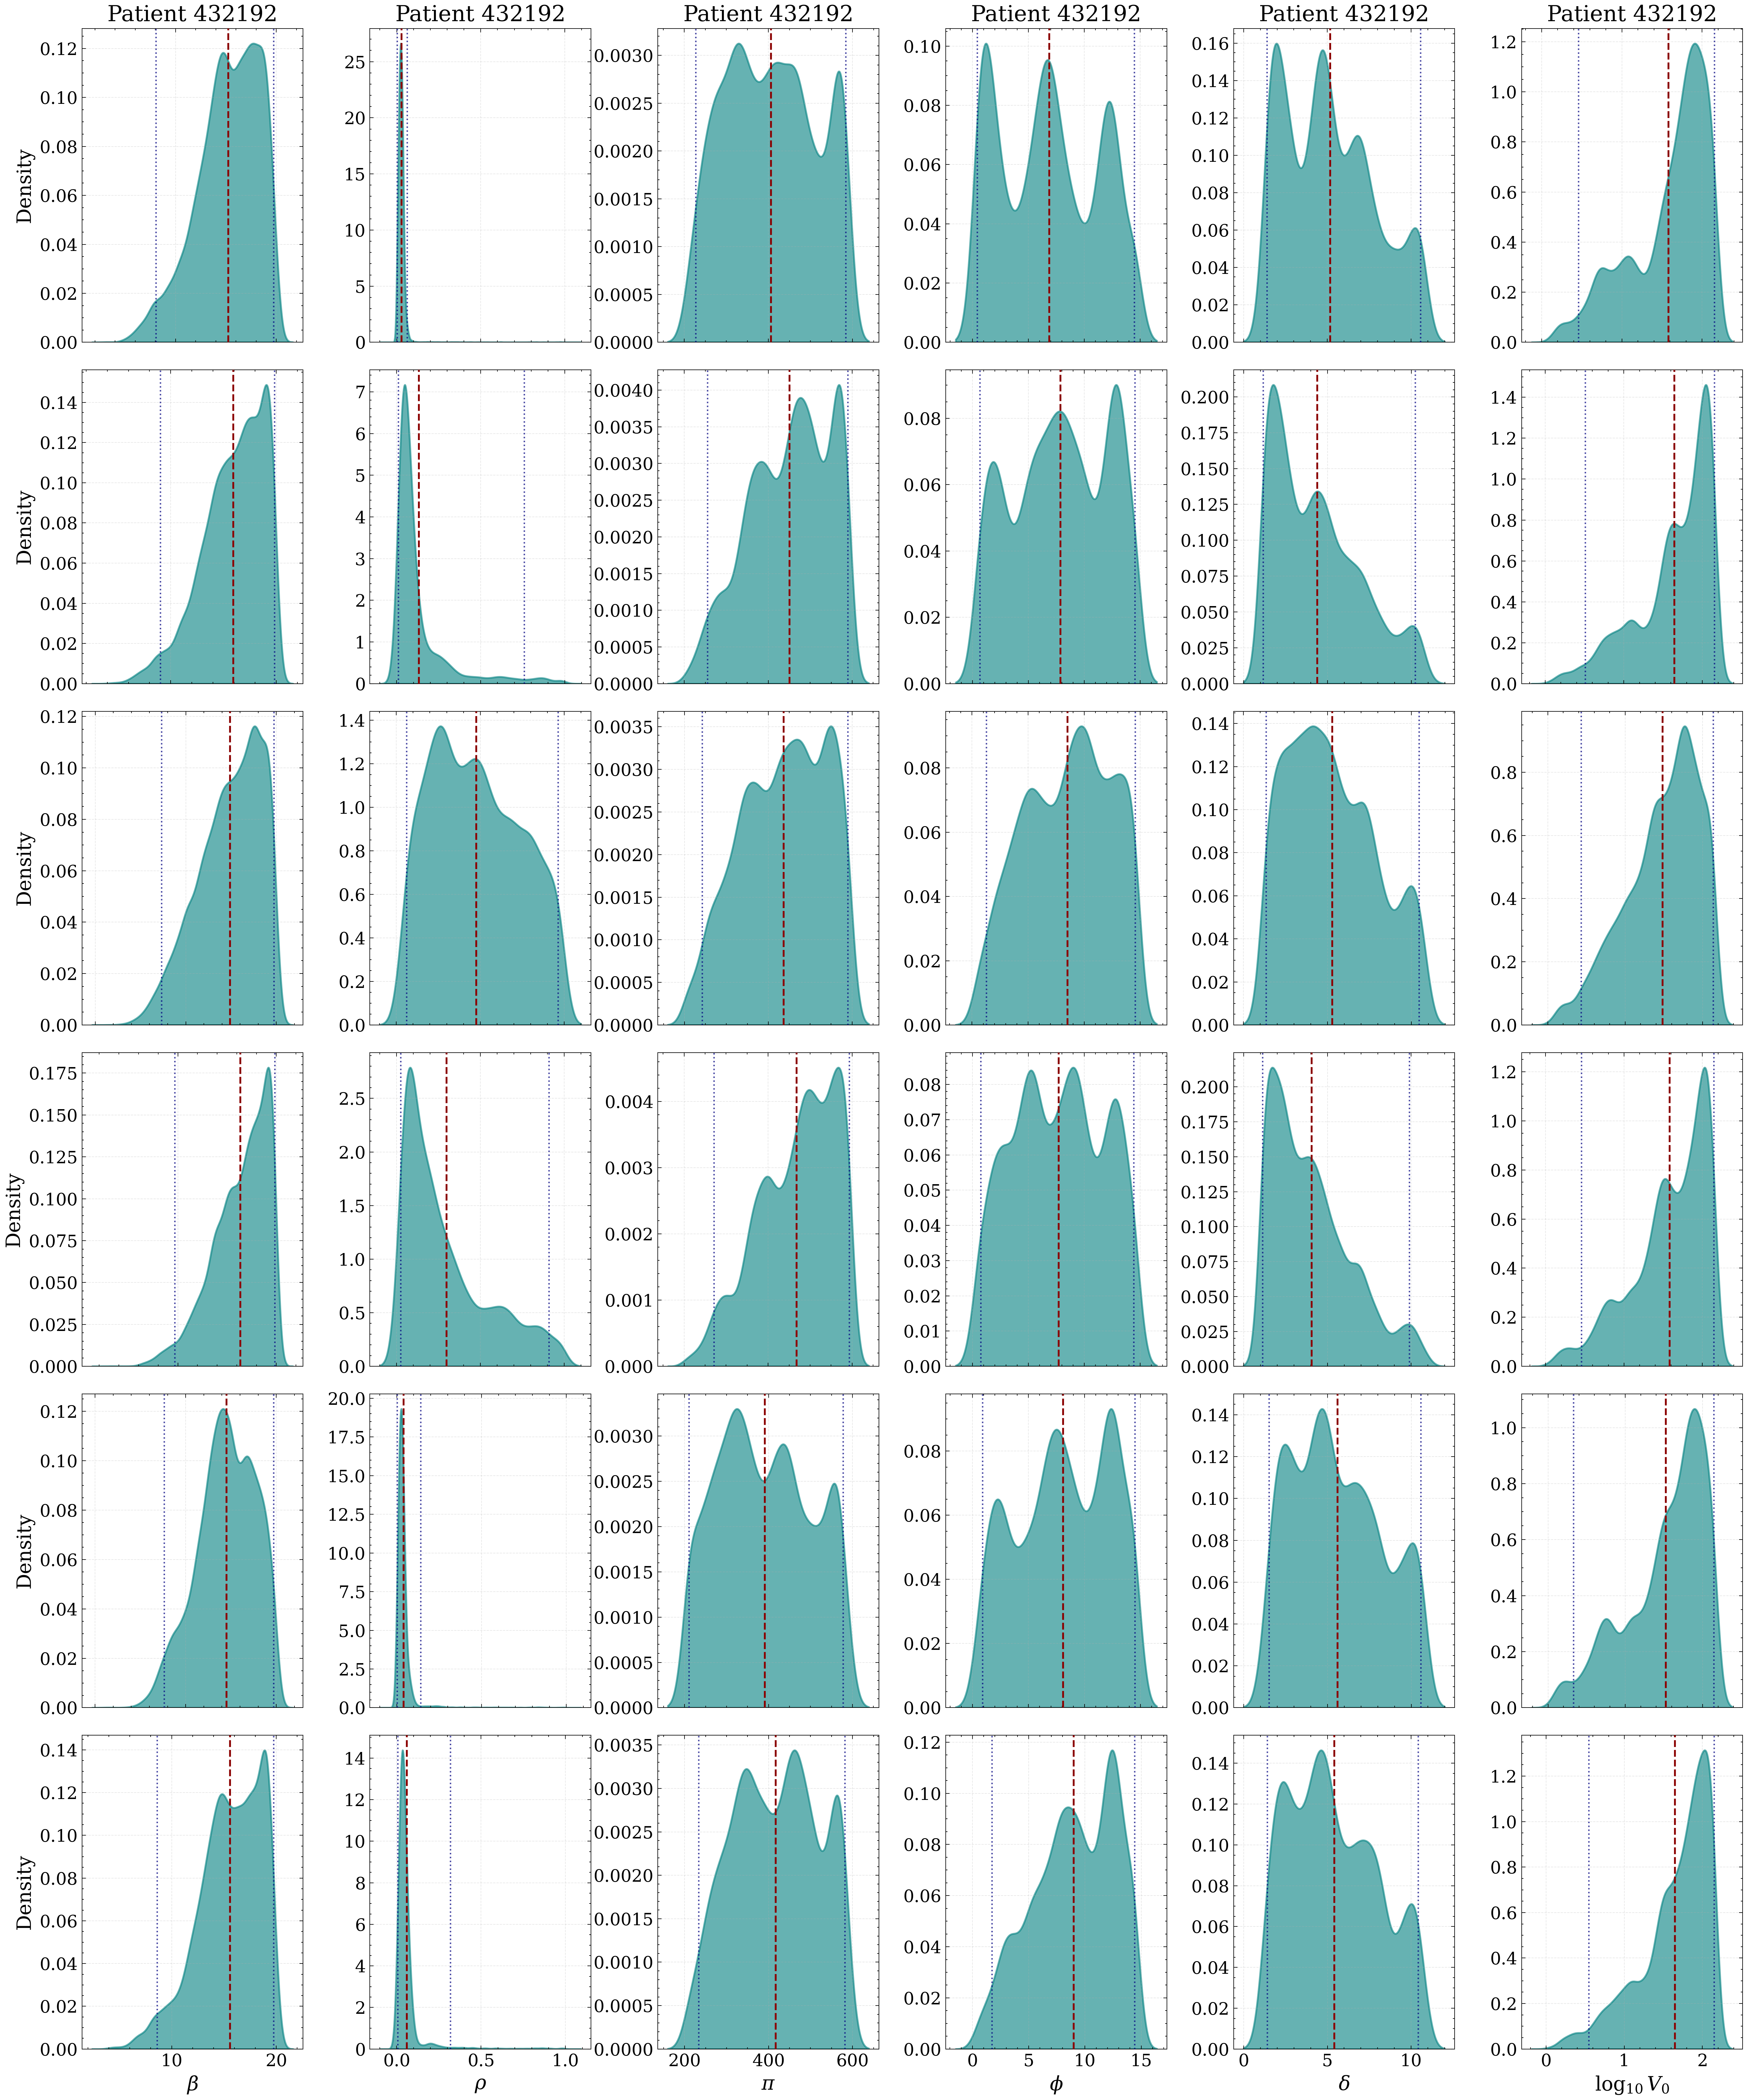
\includegraphics[width=\textwidth]{images/marginalised_posteriors.png}
\caption{\todo{Same patient ID across all figures. Add IDs along rows as mentioned in the caption.} Marginalised posterior distributions for viral dynamics parameters across six participants. Rows correspond to individual patients (IDs indicated on the right), and columns represent the inferred model parameters: transmission rate ($\beta$), eclipse phase rate ($\rho$), viral production rate ($\pi$), infected cell clearance ($\delta$), and the initial viral load ($\log_{10} V_0$). The filled teal areas represent kernel density estimates (KDE) of the 10,000 posterior samples generated via Neural Posterior Estimation. The red dashed vertical line indicates the posterior mean, while the navy dotted lines mark the 95\% credible interval. The results highlight substantial inter-patient heterogeneity, particularly in viral clearance ($\delta$) and production ($\pi$) rates, justifying the use of hierarchical or individual-level inference over population averages.}
    \label{fig:posteriors}
\end{figure}


\begin{figure}
    \centering
    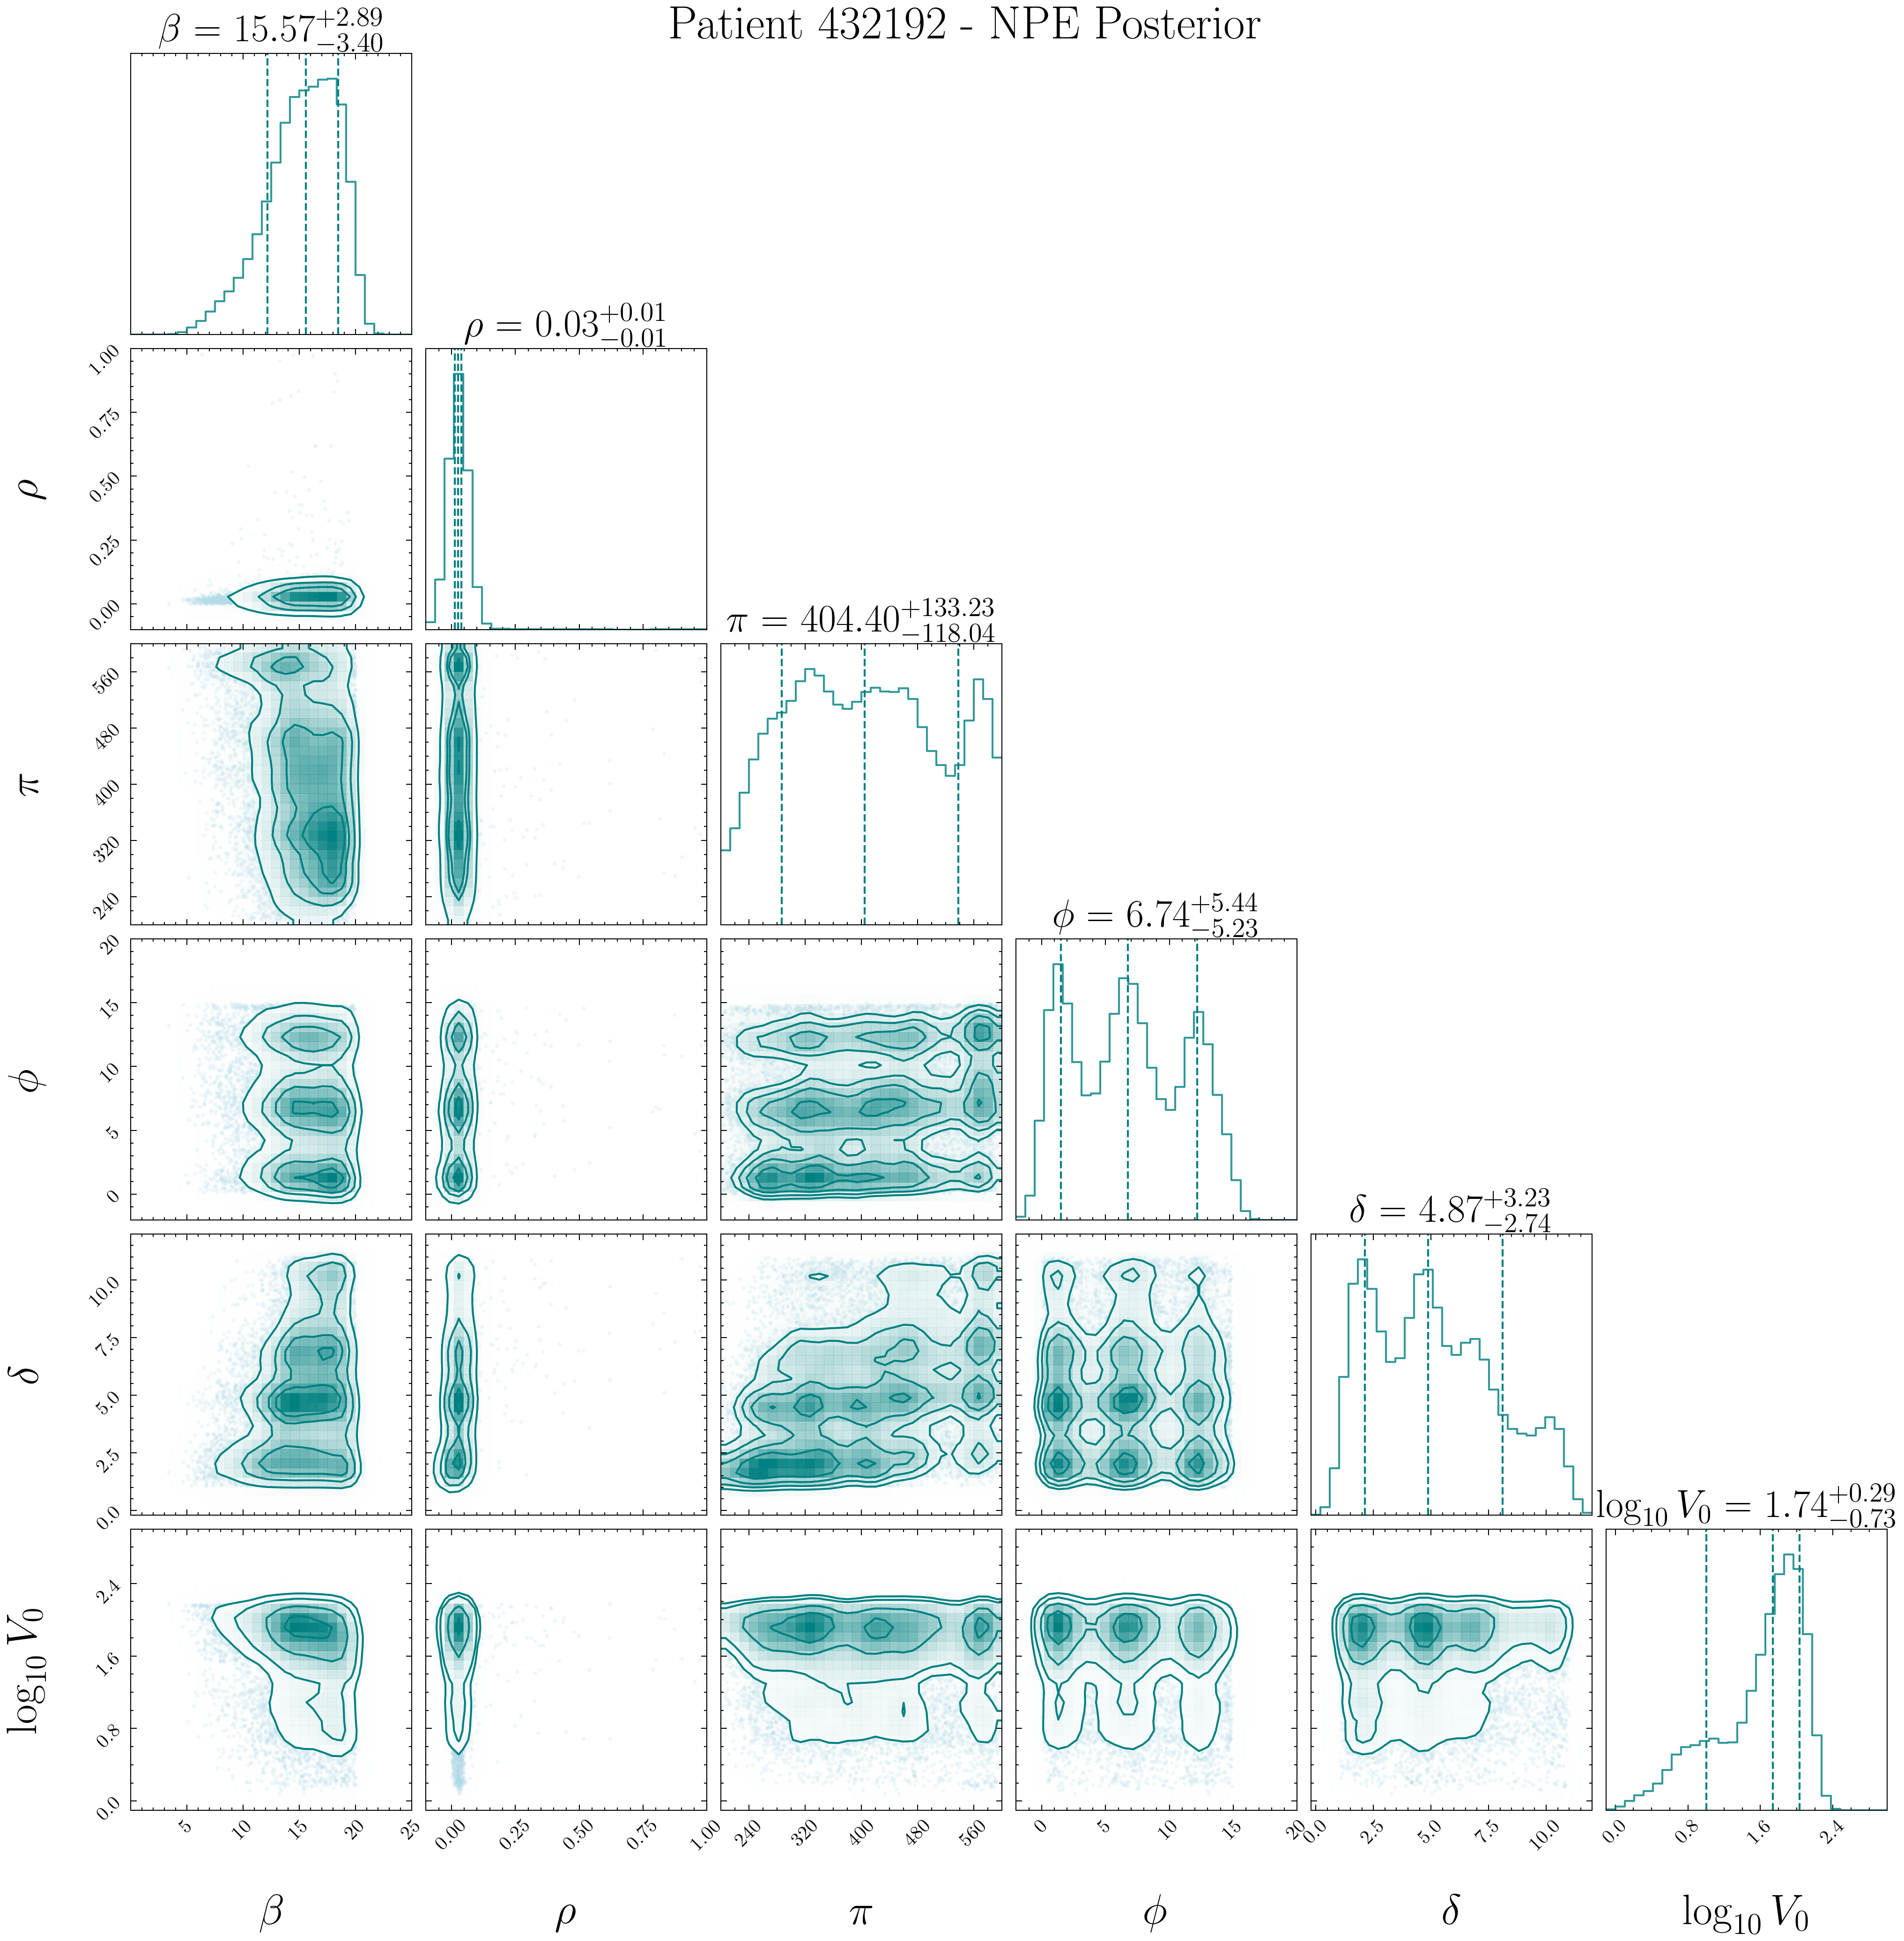
\includegraphics[width=\textwidth]{images/corner_plot_npe_canonical.png} 
\caption{Bivariate posterior distributions (corner plot) for a representative patient using our JSF-NPE framework. The diagonal panels display the univariate marginal distributions for each parameter. The off-diagonal panels show the pairwise joint distributions, with contours representing the 50\% and 95\% highest density regions. The presence of strong correlations (non-axis-aligned shapes) between parameters demonstrates that the neural network has successfully learned the complex dependency structure of the posterior, capturing the structural identifiability trade-offs inherent in the viral kinetics model.}
    \label{fig:corner_plot}
\end{figure}



\begin{figure}[htbp]
    \centering
    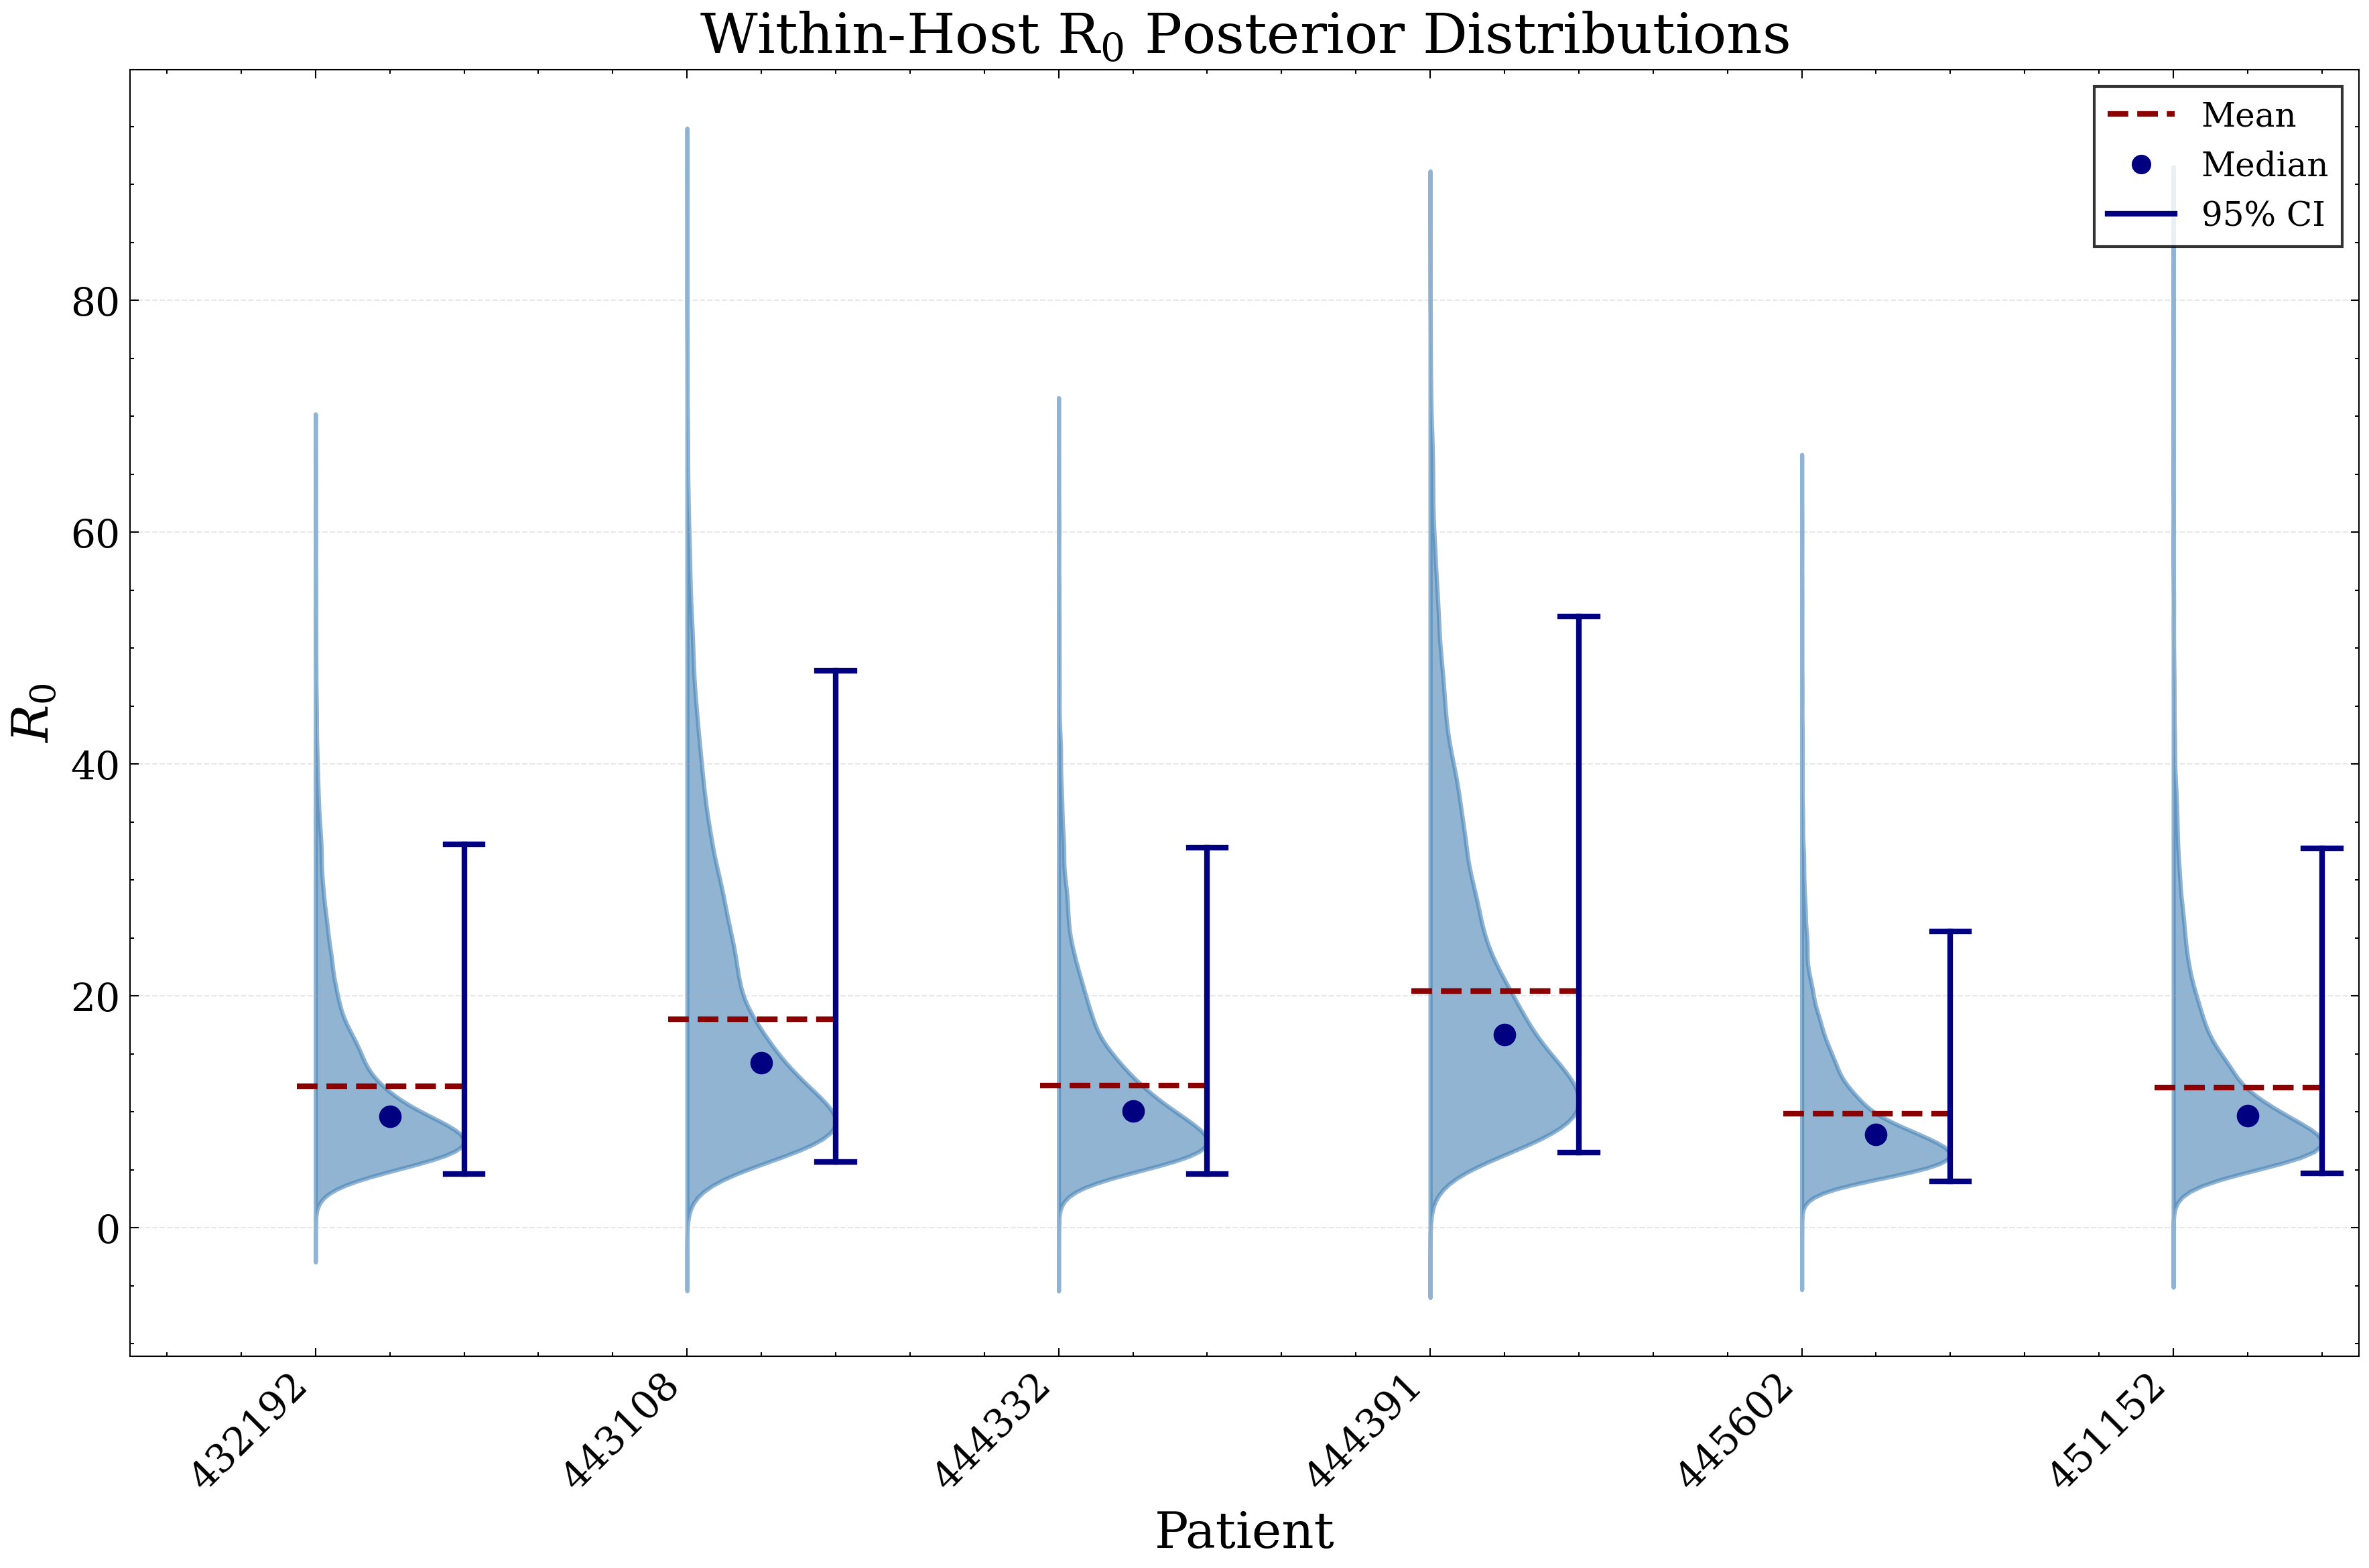
\includegraphics[width=\textwidth]{images/r0_distribution_halfviolin_canonical}
\caption{\todo{The caption needs update.} Derived posterior distributions of the basic reproduction number ($R_0$) for the cohort. $R_0$ was calculated for each posterior sample as a compound parameter of the inferred kinetics (where $R_0 \propto \beta \pi / \delta$). The half-violin plots visualize the full density of the distribution, while the internal boxplots indicate the median (white dot), interquartile range (thick bar), and $95\%$ range (thin line). While individual kinetic parameters vary significantly between patients (see Figure \ref{fig:posteriors}), the aggregate measure of viral fitness ($R_0$) remains relatively constrained across the cohort.}
    \label{fig:violins}
\end{figure}









\subsection{Benchmarking against Sequential Monte Carlo}
To validate the performance of the JSF-NPE framework, we benchmark it against a standard Sequential Monte Carlo (SMC) particle filter, which serves as the gold standard for inference in non-linear stochastic models. This comparison focuses on two critical metrics: posterior fidelity and computational efficiency. First, we assess whether the neural network accurately recovers the complex geometry of the true posterior distribution, including the parameter correlations inherent in viral dynamics. Second, we compare the runtime costs of both methods to demonstrate the practical advantages of amortized inference for clinical applications.

\subsubsection{Posterior Fidelity}

We used the SMC baseline to generate reference posterior samples for the same six patients. To quantify the fidelity of our neural approximation, we compared the JSF-NPE posteriors (Figure \ref{fig:corner_plot}) against the reference SMC samples, which are presented in Figure \ref{fig:corner_particlefilter}. Qualitatively, visual inspection of the two figures reveals a strong structural alignment between the methods across the majority of the parameters. Like the SMC baseline, the NPE method successfully captures the complex, non-linear correlations between parameters. This alignment is particularly evident in the core kinetic parameters (i.e., those which dictate the macroscopic geometry of the infection curve) $\beta$, $\pi$, and $V_0$. To quantify this similarity, we calculated the Wasserstein distance, normalised by the prior width, for the one-dimensional marginal posteriors of each parameter. The low relative Wasserstein distances for these parameters (Table \ref{tab:wasserstein_scores}) confirm that the inference network has learned the global geometry of the posterior distribution and accurately recovers the identifiable manifolds found by the particle filter. Additional discussion on the Wasserstein distance can be found in Appendix \ref{sec:wasserstein}.


While the general contours agree, there are some notable discrepancies between the particle filter and the NPE results: 
\begin{enumerate}
\item \textbf{Multimodality and Complex Correlations:} The NPE posteriors exhibit superior resolution in handling multimodal regions (e.g. parameters $\phi, \delta$). As detailed in Section \ref{sec:identifiability}, the neural network successfully resolved distinct modes that the particle filter struggled to explore effectively (likely due to particle degeneracy or local trapping in these high-curvature regions).

\item \textbf{Parameter Constraints:} Certain parameters, such as the eclipse phase rate ($\rho$), appeared consistently broader (less constrained) in the SMC results. The NPE posteriors, conversely, were able to constrain these parameters to tighter physiologically plausible ranges. We hypothesize that the network is better able to extract subtle signal features from the time series that are lost in the stochastic variance of the particle filter (discussed further in Section \ref{sec:identifiability}).

\item \textbf{Constraint on the Eclipse Phase ($\rho$):} A significant discrepancy is observed in the eclipse phase parameter ($\rho$). The SMC baseline yields a broad, uninformative posterior for $\rho$, suggesting the parameter is practically unidentifiable via the particle filter in this regime. Conversely, the NPE posteriors produce a much tighter, well-constrained distribution. This is discussed further in Section \ref{sec:param_sensitivity}.
\end{enumerate}. \textcolor{red}{TK: we should probably extend the analysis to the rest of the patient cohort, but currently only have particle filter results for one patient. It will be too much to put all corner plots here - they can go in appendices. We just require a broader statement here along the lines of "similar results are seen across the patient cohort cf identifiability and multimodality" }

\begin{figure}[htbp]
\centering
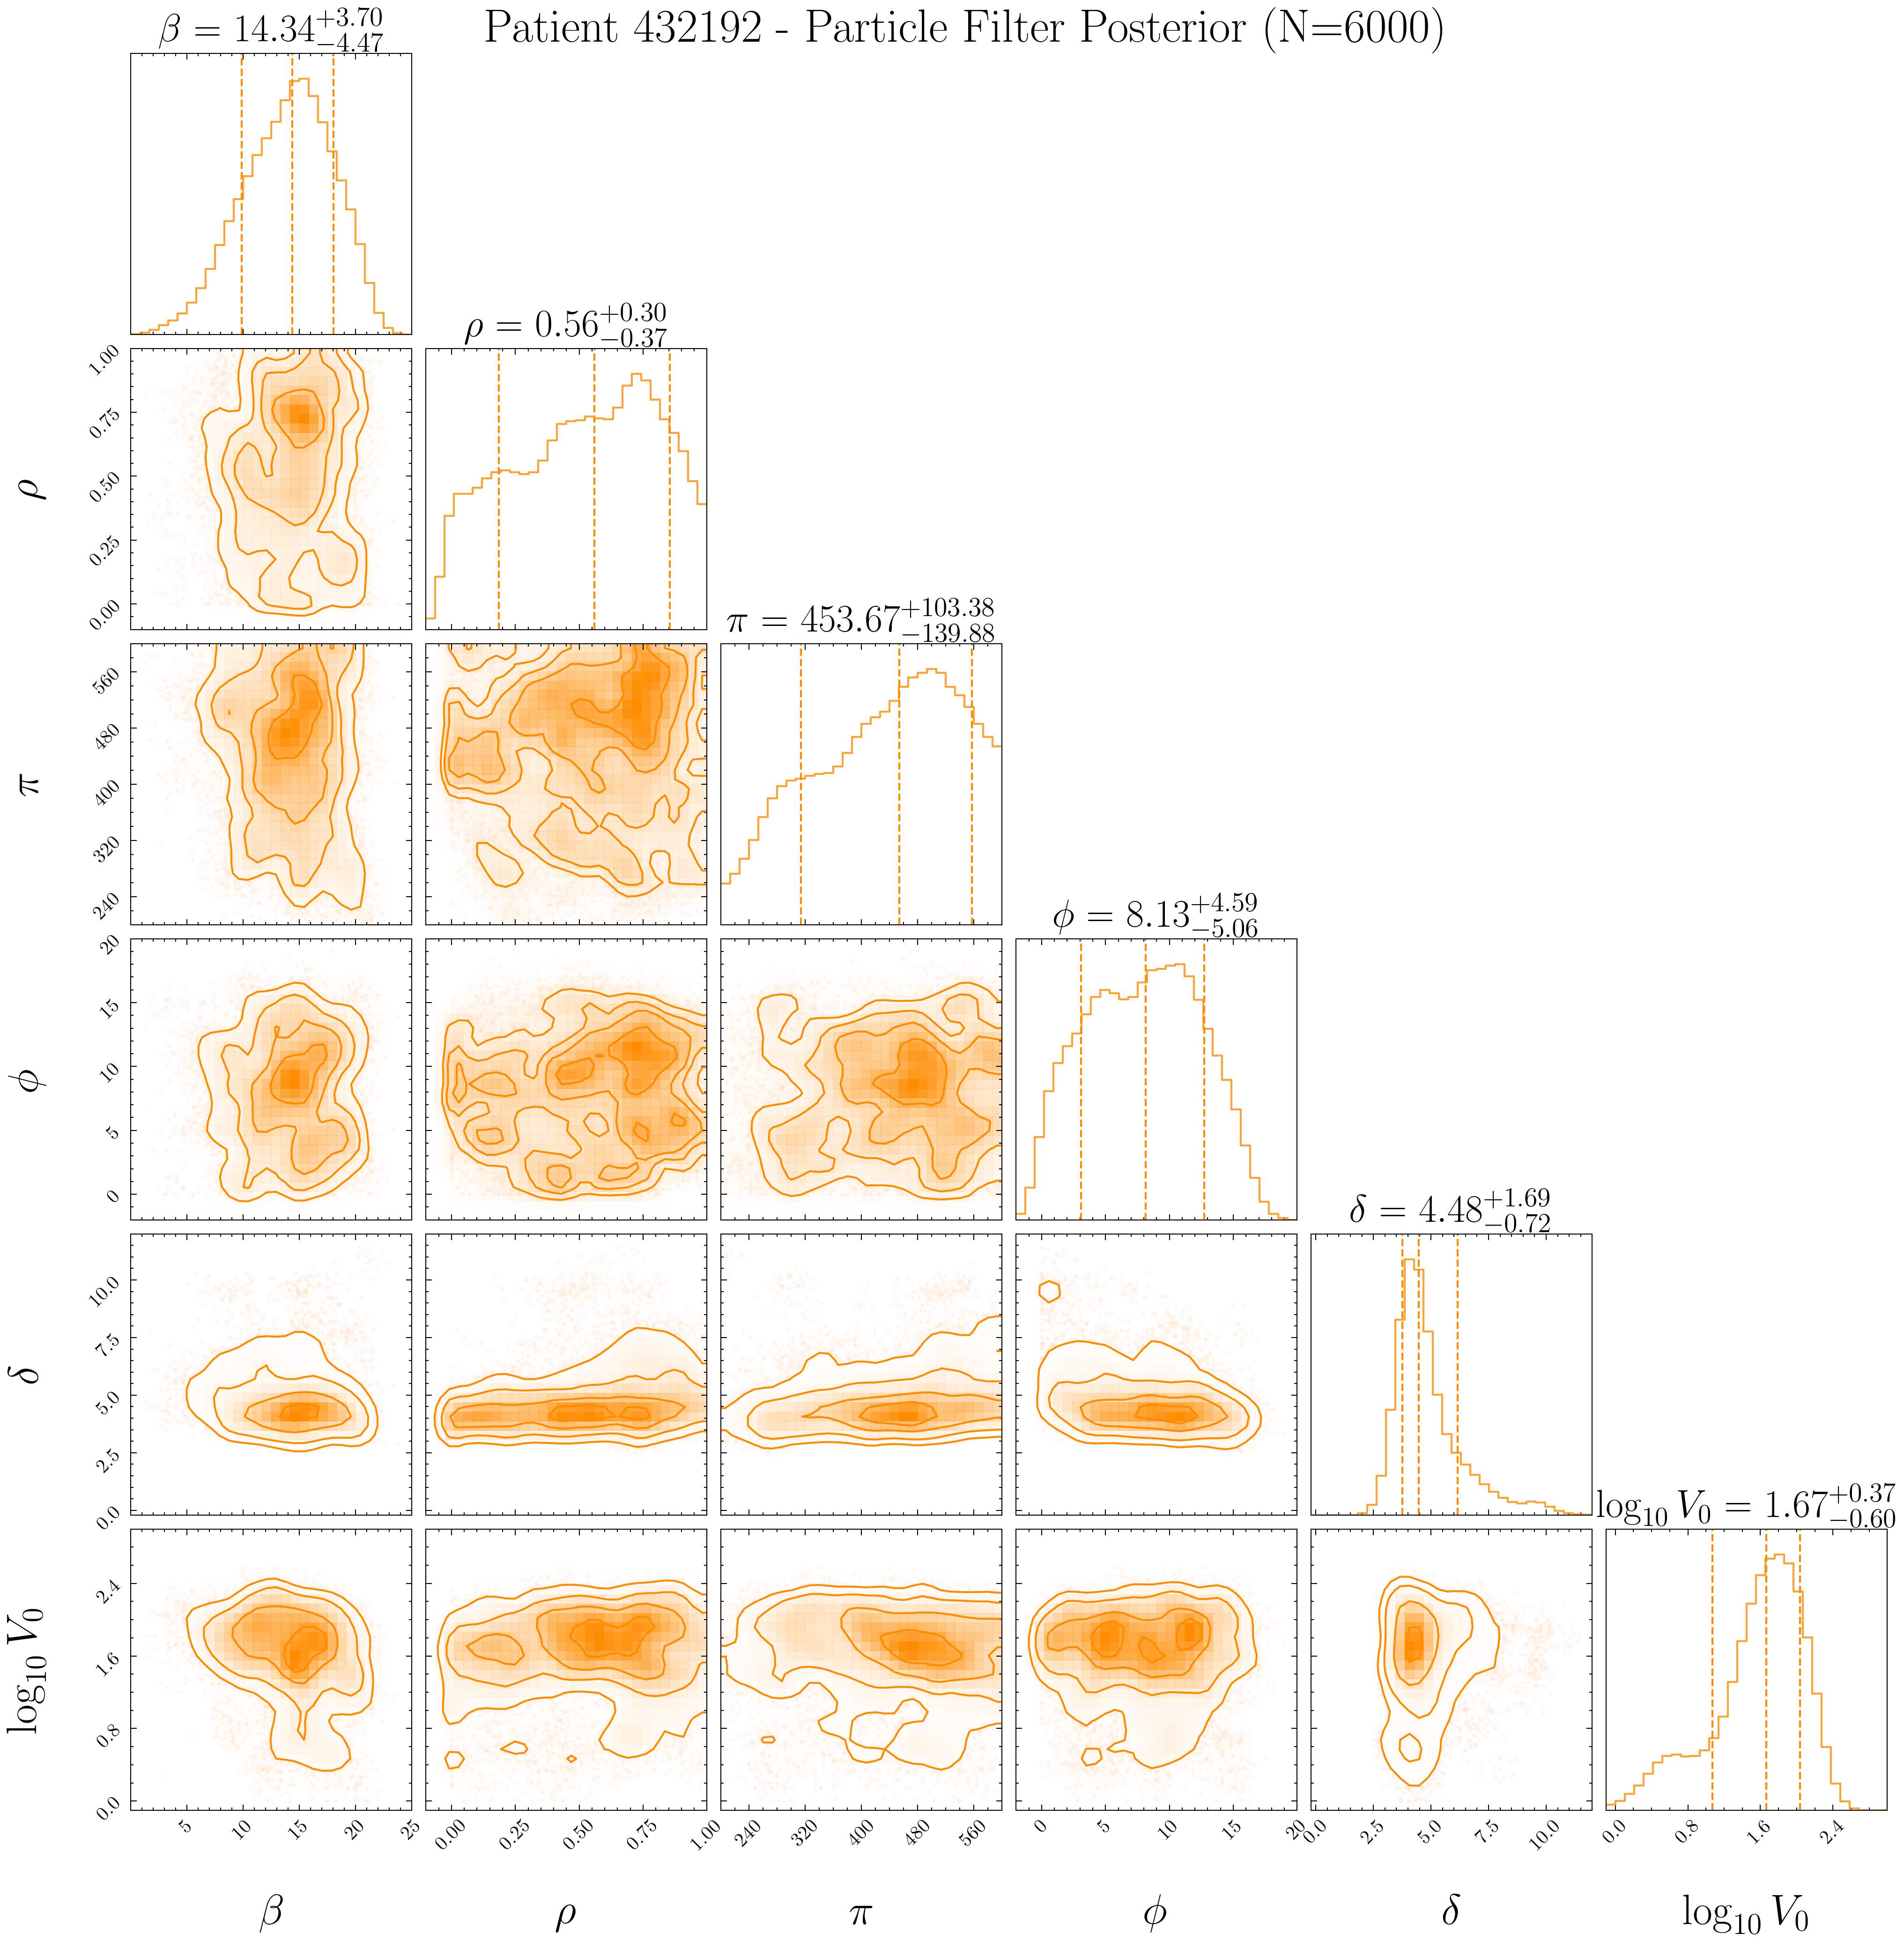
\includegraphics[width=\textwidth]{images/corner_plot_pf_canonical.png}
\caption{Posterior distributions generated by the Sequential Monte Carlo (SMC) baseline \cite{Germano2024JSF} for the representative patient shown in Figure \ref{fig:corner_plot}. While the SMC method recovers the general structure of the posterior (including the $\beta$-$\delta$ correlation), it exhibits higher variance and lower resolution in constrained parameters (e.g., $\rho$) compared to the Neural Posterior Estimation (NPE) results. This comparison highlights the ability of NPE to provide high-fidelity inference without the sampling noise associated with finite-particle approximations.}

\label{fig:corner_particlefilter}

\end{figure}

\begin{table}[htbp]
\centering
\caption{\textbf{Quantitative Comparison of Posterior Distributions.} Normalised Wasserstein distance ($W_1$) between the 1D marginal posteriors of the NPE and the SMC baseline for patient 432192, cf. Figures \ref{fig:corner_plot}, \ref{fig:corner_particlefilter}. Low values for the core kinetic parameters ($\beta, \pi, V_0$) indicate strong distributional agreement. The higher distance for $\rho$ reflects the difference in posterior width, where NPE successfully constrained the parameter while the SMC baseline remained uninformative.}
\begin{tabular}{c c}
\toprule
\textbf{Parameter} & \textbf{Wasserstein Dist. (Normalised)} \\
\midrule
$\beta$       & 0.0694 \\
$\rho$         & 0.5099 \\
$\pi$       & 0.0890 \\
$\phi$            & 0.0744 \\
$\delta$      & 0.1267 \\
$\log_{10}V_0$  & 0.0253 \\
\bottomrule
\end{tabular}
\label{tab:wasserstein_scores}
\end{table}



\subsubsection{Computational Efficiency}\label{sec:computation_time}

A summary of the computational costs for the NPE and SMC methods is presented in Table \ref{tab:runtime}. The SMC baseline represents an online inference method, where the heavy computational burden of differential equation integration is repeated entirely for every new observation sequence. In contrast, the JSF-NPE method utilizes an amortized inference strategy, incurring a fixed upfront cost while rendering subsequent inference steps negligible. This structural difference addresses the two critical bottlenecks identified in Section \ref{sec:introduction}: latency for time-sensitive intervention and throughput for large-scale analysis.

Regarding latency, the particle filter required $\approx 5$ hours per patient to compute the posterior distributions shown in Figure \ref{fig:corner_particlefilter}. Conversely, the NPE network reduced inference latency to $< 1$ second per patient.

Regarding throughput, the SMC baseline scales linearly with the number of patients. For the current cohort of six patients, this required a total of $\approx 30$ hours ($6 \times 5$ h). This linear scaling becomes prohibitive for larger datasets; for a hypothetical cohort of 100 patients, SMC would require $\approx 500$ compute hours. The NPE framework, having already incurred the fixed training cost, can process a 6-patient or 100-patient cohort without any additional simulation overhead.


\begin{table}[htbp]
\centering
\caption{Comparison of computational resources. Times are reported in hours (h). The JSF-NPE method resolves both the throughput and latency bottlenecks: the fixed training cost enables scalable population analysis, while the sub-second inference time enables real-time clinical application.}
\label{tab:runtime}
\begin{tabular}{@{}lccc@{}}
\toprule
\textbf{Method} & \textbf{Fixed Training Cost} & \textbf{Inference Latency (Per Patient)} & \textbf{Total (6 Patients)} \\
\midrule
SMC (Particle Filter) & N/A & $\approx 5.0$ h & $\approx 30.0$ h \\
JSF-NPE (Ours) & $\approx 2.5$ h & \textbf{$<$ 1 second} & $\mathbf{\approx 2.5}$ \textbf{h} \\
\bottomrule
\end{tabular}
\end{table}





\section{Discussion}

\subsection{Identifiability}\label{sec:identifiability}

A key finding of this study is the ability of the neural framework to resolve features of the posterior landscape that sequential methods miss. This advantage stems from a fundamental algorithmic distinction: while Sequential Monte Carlo (SMC) explores the parameter space locally via stepwise propagation, JSF-NPE learns a global mapping from data to parameters. Indeed, the particle filter is ostensibly a method for state-space estimation in filtering problems, rather than a parameter estimation method \textit{per se}. Adapting it for static inference (e.g., via state augmentation or jittering) often introduces inefficiencies when exploring complex, fixed parameter landscapes. This difference manifests in two critical areas: the resolution of multimodality and correlations, and the sensitivity to late-stage dynamics.



Regarding multimodality, as noted in Section \ref{sec:results}, NPE identified multimodal structures in the immune signaling ($\phi$) and clearance ($\delta$) parameters, whereas the particle filter often collapsed to a single mode. This multimodality is mechanically consistent with the TEIRV model structure, described in Appendix \ref{sec:teivr_identifiable}. The SMC approach is path-dependent; early resampling steps often cause the particle population to "commit" to one mode (e.g., high-$\delta$) and lose the diversity required to represent the alternative mechanism (mode collapse). NPE, by training on the full prior predictive distribution, successfully preserves this global topology.





Regarding late-stage dynamics, while the JSF-NPE framework consistently yields peaked, informative posteriors for $\rho$, SMC baseline frequently returns broad distributions resembling the prior. This discrepancy highlights a fundamental, yet often overlooked, distinction between \textit{structural} identifiability (a property of the equations) and \textit{algorithmic} identifiability (a property of the inference engine). Biologically, $\rho$ governs the return of refractory cells to the susceptible state. This feedback loop is a "late-acting" mechanism; its influence on viral load is negligible during the exponential growth phase and only becomes dynamically relevant in the tail of the infection, after a significant population of refractory cells ($R$) has accumulated. The SMC algorithm struggles in this domain due to particle degeneracy a known pathology in Sequential Monte Carlo methods applied to static parameter inference \cite{Andrieu2010, Kantas2009}. In an SMC framework, particles are resampled at every time step based on their likelihood weights. During the early days of the infection ($t=1 \dots 5$), the likelihood function is almost perfectly flat with respect to $\rho$ (since $\partial V / \partial \rho \approx 0$). However, the resampling step introduces stochastic noise. Particles with different $\rho$ values are selected or discarded purely based on their fit to other, active parameters (like $\beta$ or $V_0$). By the time the simulation reaches the late phase ($t > 10$) where $\rho$ actually exerts an influence on the trajectory, the population of particles often shares a single common ancestor from the early time steps. The diversity of $\rho$ values has been "resampled away" before the data could inform them. The resulting posterior is broad not because the data lacks information, but because the algorithm discarded that information during the sequential pass. In contrast, the JSF-NPE framework is a global inference method. The neural network processes the entire time-series (or a summary embedding thereof) simultaneously to map the observation $x$ to the parameter $\theta$. It does not suffer from sequential attrition. The network learns during the training phase that subtle curvature changes in the tail of the trajectory are distinct signatures of $\rho$, allowing it to utilize information from day 14 just as effectively as information from day 1. This result is important for multiscale modellers  A broad posterior is typically interpreted as a sign of insufficient data (practical non-identifiability) or redundant parameterization (structural non-identifiability). Our findings suggest a third possibility: that the chosen inference algorithm is lossy. In the context of viral dynamics, global amortized methods may be strictly superior over sequential methods for estimating parameters that govern late-stage feedback loops or immune memory.

\subsection{Utility in Clinical and Epidemiological Settings}\label{sec:clinical_implications}

The computational efficiency demonstrated in Section \ref{sec:computation_time} has  implications for the practical deployment of viral dynamic models.

In acute clinical settings, such as managing immunocompromised patients or optimizing antiviral dosing in the ICU, latency is the limiting factor. Standard inference methods that require hours of computation are effectively "post-mortem" tools—useful for retrospective analysis but too slow for real-time decision support. The sub-second inference capability of the trained NPE network allows for interactive medicine. Clinicians could potentially update parameter estimates instantaneously as new viral load measurements arrive, enabling adaptive therapy protocols that respond to the patient's specific clearance rates ($\delta$) or immune status ($\phi$) in real-time.

In epidemiological contexts, the bottleneck shifts to throughput. Analysing large cohorts to track population-level shifts—such as the emergence of drug-resistant strains or evolving infectivity ($\beta$) profiles—requires processing thousands of infection chains. The linear scaling of SMC makes such analyses computationally prohibitive. The amortized cost structure of NPE, however, renders large-scale surveillance feasible. Once the network is trained, it can be applied to thousands of patient datasets with negligible marginal cost, effectively bridging the gap between detailed within-host mechanistic modeling and broad population-level epidemiology.




\subsection{Code Availability}
The code for JSF simulation, NPE training, and analysis is be made available at \textcolor{red}{TK: links to be added. Might be best to merge current fork back into JSFGermano2024? Or do we spin out a standalone repo?}



\section{Acknowledgment}
This research was supported by The University of Melbourne’s Research Computing Services and the Petascale Campus Initiative. \textcolor{red}{TK: any other funding or acknowledgements to go here}

\bibliographystyle{unsrt}
\bibliography{references}  


\appendix



\appendix
\section{Posterior Predictive Checks} \label{app:ppc}
\textcolor{red}{TK: somewhat optional since we are focusing on the comparison with PF, rather than NPE as a standalone tool. Might be good to have for thoroughness, but if paper starts to get too long it is probably fine to drop}


To further validate the goodness-of-fit of the JSF-NPE framework, we performed posterior predictive checks (PPC). For each patient, we drew parameter sets from the inferred posterior distributions (presented in Section \ref{sec:results}) and simulated the corresponding trajectories using the JSF algorithm. 

Figure XX compares these simulated trajectories against the observed clinical Cycle Number (CN) data (converted to $\log_{10}$ viral load). The shaded regions represent the 95\% credible intervals of the predictive distribution.

The results demonstrate...



\section{Wasserstein distance} \label{sec:wasserstein}



\textcolor{red}{TK: Short notes on Wasserstein distance (which may be unfamiliar to readers), why its preferred to KL, and relevant references}

\section{Full Posterior Corner Plots}

In the main text (Figure \ref{fig:comparison_corner}), we presented the joint posterior distribution for a representative patient. For completeness, we present the full corner plots for the remaining five subjects in Figures \ref{fig:supp_corner_2} through \ref{fig:supp_corner_6}. 

\textcolor{red}{TK: all corner plot figures for NPE and PF to go here. This will take up a lot of space, so maybe throw this appendix right at the end}

% Repeat for Patients 3-6...

\section{Mathematical Analysis of Structural Identifiability}\label{sec:teivr_identifiable}

\textcolor{red}{TK: TBD. Needs some cleaning up. Main point is that we can tell just by looking at the equations that some multimodal structure should be recovered by the inference engine}


The peak viral turnover is driven by the depletion of the effective replicative pool, which can occur via two distinct mechanisms. The first mechanism is when $\phi$ is large, target cells are rapidly converted into the refractory state, limiting the substrate for infection. The second mechanism is when $\delta$ is high, ther eis a rapid death of infectious disease cells reducing the source of new virions 


The multimodal posterior distributions observed in the NPE results (particularly for $\phi$ and $\delta$) and the strong correlation ridges (e.g., between $\beta$ and $\delta$) can be understood analytically by examining the deterministic limit of the TEIRV system.

We begin with the observation that viral turnover (the peak) occurs when the effective reproduction number drops below unity. To elucidate the mechanisms driving this, we apply a Quasi-Steady State Assumption (QSSA) to the fast-variable equations. Since viral dynamics are typically faster than cellular dynamics, we assume $dV/dt \approx 0$ relative to cell changes, yielding the proportionality:
\begin{equation}
    V(t) \approx \frac{\pi}{\gamma} I(t)
\end{equation}
Substituting this relationship into the governing equation for Target cells ($T$), we obtain:
\begin{align}
    \frac{dT}{dt} &= \rho R - \beta T V - \phi I T \\
    &\approx \rho R - \beta T \left( \frac{\pi}{\gamma} I \right) - \phi T I \\
    &= \rho R - \left( \frac{\beta \pi}{\gamma} + \phi \right) T I \label{eq:lumped}
\end{align}
In the acute phase of infection (where $\rho R$ is negligible), the depletion of target cells is governed by the lumped effective rate constant:
\begin{equation}
    \mathcal{K}_{\text{depletion}} = \frac{\beta \pi}{\gamma} + \phi
\end{equation}
Equation \ref{eq:lumped} reveals a fundamental structural non-identifiability: the data observes the rate of viral decline, which correlates with the rate of target cell depletion. However, this depletion can be achieved either by a high infection rate ($\beta$) generating new infectious centers, or by a high immune signaling rate ($\phi$) rendering cells refractory.

Any combination of parameters satisfying $\frac{\beta \pi}{\gamma} + \phi = C$ (for some constant $C$ determined by the observed trajectory slope) will result in a nearly identical $T(t)$ profile, and consequently, a nearly identical $V(t)$ trajectory. This linear constraint explains the correlation ridge observed in the posterior distributions.

Furthermore, we consider the condition for the viral peak. The peak occurs when the effective reproduction number $R_{\text{eff}}(t) = 1$. In the standard TIV model limit, this is given by:
\begin{equation}
    R_{\text{eff}}(t) = \frac{\beta \pi T(t)}{\delta \gamma} \approx 1 \implies T_{\text{peak}} \approx \frac{\delta \gamma}{\beta \pi}
\end{equation}
This imposes a second constraint: the remaining target cell population at the peak ($T_{\text{peak}}$) is determined by the ratio $\delta / \beta$.

Thus, the inference problem faces a "balancing act" defined by two coupled constraints:
\begin{enumerate}
    \item The \textbf{Slope Constraint}: $\frac{\beta \pi}{\gamma} + \phi \approx \text{const}$ (governing the speed of target burnout).
    \item The \textbf{Peak Constraint}: $\frac{\delta}{\beta} \approx \text{const} \times T_{\text{peak}}$ (governing the turnaround point).
\end{enumerate}

The Particle Filter, due to its sequential greedy nature, tends to latch onto a single solution satisfying these constraints (e.g., High $\delta$, Low $\phi$). In contrast, the JSF-NPE network, trained globally, identifies the full manifold of solutions. It reveals that the data can be explained equally well by a "Cell Death" model (High $\delta$, High $\beta$, Low $\phi$) or an "Immune Suppression" model (Low $\delta$, Low $\beta$, High $\phi$), resulting in the multimodal posteriors seen in Figure \ref{fig:posteriors}.


\begin{enumerate}
    \item \textbf{Target Limitation (High $\phi$):} rapid conversion of target cells into the refractory state, limiting the substrate for infection.
    \item \textbf{Source Clearance (High $\delta$):} Rapid death of infectious cells, reducing the source of new virions.
\end{enumerate}
Since the observation model tracks only viral load ($V$) and not cellular compartments, these mechanisms create a "ridge" of structural unidentifiability. 




\end{document}





% \textbf{Settings requiring rapid per-case inference:}

% \begin{itemize}
% \item \textbf{Antiviral treatment optimization}: A physician selecting between treatment regimens, adjusting dosing schedules, or predicting treatment failure must make decisions within clinical consultation timeframes. Real-time parameter estimation from early viral load measurements could guide personalized treatment strategies, but waiting hours or days for inference results is clinically impractical.

% \item \textbf{Immunocompromised patient management}: ICU, transplant, or chemotherapy patients experiencing viral infections exhibit highly variable viral dynamics and face elevated risks. These cases require rapid, frequent parameter updates as patient status changes, where slow inference methods delay time-sensitive treatment decisions.

% \item \textbf{Outbreak detection and characterization}: When the first suspected case of a novel pathogen or livestock disease is detected, rapid parameter estimation is critical to confirm whether an outbreak is occurring and characterize its transmission potential. Hours of delay in analyzing initial cases can determine whether containment is feasible.
% \end{itemize}

% \textbf{Settings requiring inference across many individuals:}

% \begin{itemize}
% \item \textbf{Outbreak response at scale}: Once an outbreak is confirmed, effective response requires analyzing viral dynamics across all detected cases---potentially hundreds of animals in a livestock epidemic (e.g., foot-and-mouth disease spreading through herds) or dozens to hundreds of human cases in an emerging infectious disease outbreak. Decisions about culling, quarantine zones, or resource allocation depend on population-level parameter estimates that cannot wait for serial inference across each individual.

% \item \textbf{Public health surveillance}: Health officials monitoring endemic disease spread across populations must analyze data from hundreds or thousands of individuals. Serial application of expensive inference methods makes large-scale analysis infeasible within relevant time frames.

% \item \textbf{Clinical trials with adaptive designs}: Adaptive trials for antivirals or vaccines require interim analyses across cohorts to make go/no-go decisions, adjust dosing, or identify efficacy signals. When each patient's data requires hours of inference time, timely interim analyses become computationally prohibitive.

% \item \textbf{Drug resistance surveillance}: Monitoring for emergence of resistant viral strains requires analyzing viral dynamics across patient populations to detect parameter shifts signaling resistance evolution. The scale of surveillance needed---potentially thousands of patients across multiple sites---is incompatible with computationally expensive inference methods.

% \item \textbf{Chronic infection management}: Patients with HIV, hepatitis C, or other chronic viral infections require repeated parameter estimation over months or years of treatment monitoring. A single patient may need analysis at dozens of clinical visits; across a cohort of hundreds of patients, the cumulative computational cost of slow inference methods becomes unsustainable for routine clinical use.
% \end{itemize}